%! TeX root = ../../main.tex

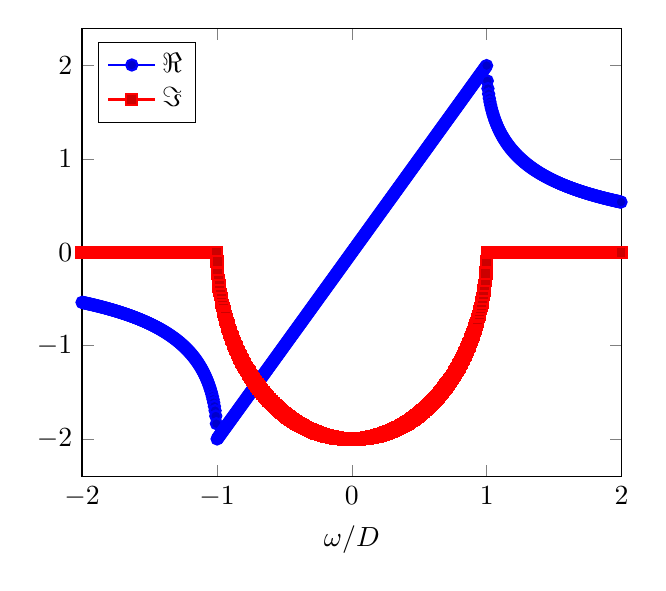
\begin{tikzpicture}
    \begin{axis}[
            xlabel=$\omega/D$,
            xmin=-2,
            xmax=2,
            every axis plot/.append style={
                    thick,
                    domain=-2:2,
                    samples=800,
                },
            legend entries={
                    $\Re$,
                    $\Im$,
                },
            legend pos=north west,
        ]

        \addplot {
            x < -1 ?
            % (-\infty, -D)
            2 * (x + sqrt(x^2 - 1))
            :
            (
            x < 1 ?
            % [-D, D)
            2 *x
            :
            % [D, \infty)
            2 * (x - sqrt(x^2 - 1))
            )
        };
        \addplot {abs(x) < 1 ? -2 * sqrt(1 - x^2) : 0};
    \end{axis}
\end{tikzpicture}
